\documentclass[a4j, titlepage]{jarticle}
\usepackage{float}
\usepackage[dvipdfmx]{graphicx}
%\usepackage{mediabb}
\makeatletter
%https://qiita.com/ta_b0_/items/2619d5927492edbb5b03
\usepackage{listings,jlisting} %日本語のコメントアウトをする場合jlstlistingが必要
\usepackage[top=30truemm,bottom=30truemm,left=25truemm,right=25truemm]{geometry}
%ここからソースコードの表示に関する設定
\lstset{
    basicstyle={\ttfamily},
    identifierstyle={\small},
    commentstyle={\smallitshape},
    keywordstyle={\small\bfseries},
    ndkeywordstyle={\small},
    stringstyle={\small\ttfamily},
    frame={tb},
    breaklines=true,
    columns=[l]{fullflexible},
    numbers=left,
    xrightmargin=0zw,
    xleftmargin=3zw,
    numberstyle={\scriptsize},
    stepnumber=1,
    numbersep=1zw,
    lineskip=-0.5ex,
    breakindent=0pt
}
%ここまでソースコードの表示に関する設定

\if0
---------------------------------こめこめこめこめこめこめこめこめこめこめこめ
\renewcommand{\thefigure}{\arabic{figure}}
\@addtoreset{figure}{section}
\makeatother
\makeatletter
\renewcommand{\thetable}{\arabic{table}}
\@addtoreset{table}{section}
\makeatother
\makeatletter
\renewcommand{\theequation}{\arabic{equation}}
\@addtoreset{equation}{section}
\makeatother
---------------------------------こめこめこめこめこめこめこめこめこめこめこめ
\fi

\usepackage{multicol}
\usepackage{okumacro}

\usepackage{amssymb}
\usepackage{amsmath}
\usepackage{url}
\usepackage{ascmac}
\usepackage{fancyvrb}
\usepackage{otf}
\usepackage{here}

\newcommand{\GitHub}{
\includegraphics[scale=0.07]{image/github.png}}
\newcommand{\VSCode}{
\includegraphics[scale=0.012]{image/vscode-icon.png}}

\title{\LaTeX の俺的最強チートシート}
\author{Bony\_Chops}


\begin{document}
\maketitle
\begin{abstract}
    ここを書くには
    \begin{lstlisting}
\begin{abstract}
    ここを書くには...
\end{abstract}
    \end{lstlisting}
\end{abstract}

\setcounter{section}{-1}
\section{はじめに}
\textbf{Hello hackers!} これから\textbf{Word}から日本語 を使い始めるキミや、ある程度日本語 には慣れたけどコマンドを忘れがちなキミに向けたチートシートです。
\subsection{付録について}
このPDFや\TeX ソース、付録に掲載しているソースは全てGitHub上で公開しています。実践する際にぜひお役立てください。\\
\GitHub BonyChops / latex-cheatsheet (\url{https://github.com/BonyChops/latex-cheatsheet})
\subsection{環境}
本チートシートは以下の環境を使っていることを想定して書いています。特殊な仕様意外は基本的に同じだと思います。

\begin{table*}[htbp]
    \center
    \caption{筆者の環境}
    \begin{tabular}{|c|c|} \hline
        OS & Ubuntu 20.04 \\ \hline
        エディタ & Visual Studio Code \\ \hline
        環境 & TeX Live 2017 \\ \hline
        コンパイルスクリプト & ptex2pdf \\ \hline
        documentclass & jarticle \\ \hline
    \end{tabular}
\end{table*}

また、本ガイドと同じ環境で行う場合、\textbf{\underline{以下のstyファイルが必要です}}。インターネットから探してきて、texファイルと同じディレクトリに置くか、\ref{sec:installSty}を参考にして、styファイルをインストールしてください。
\begin{itemize}
    \item jlisting.sty
\end{itemize}

\newpage

\section{コマンド集}
いっぱいあります。載せる順番は適当です。

\subsection{章 $\cdot$ 節 $\cdot$ 項 を構成する $\cdots$ \textbackslash section $\cdot$ \textbackslash subsection $\cdot$ \textbackslash subsubsection}

章 $\cdot$ 節 $\cdot$ 項 を構成する

\subsubsection{レポート風}
\begin{multicols}{2}

\subsubsection*{コマンド}

\begin{lstlisting}
\section{目的}
今回はりんごの剥き方を理解することを目的とする。

\section{理論}
本章では本実験に必要な理論をまとめる。

\subsection{包丁について}
本節では包丁についてをまとめる。

\subsubsection{さばき方}
本項では $\cdots$
\end{lstlisting}

\vfill\null
\columnbreak

\subsubsection*{実行結果}
\setcounter{section}{0}
\begin{screen}

    \section{目的}
    今回はりんごの剥き方を理解することを目的とする。

    \section{理論}
    本章では本実験に必要な理論をまとめる。

    \subsection{包丁について}
    本節では包丁についてをまとめる。

    \subsubsection{さばき方}
    本項では $\cdots$

\end{screen}


\end{multicols}
\setcounter{section}{1}
\subsubsection{番号をなくす}
コマンドの最後に*をつけよう

\begin{multicols}{2}

\subsubsection*{コマンド}

\begin{lstlisting}
\section{番号ありの章}
\subsection{番号ありの節}
\subsubsection{番号ありの項}

\section*{番号なしの章}
\subsection*{番号なしの節}
\subsubsection*{番号なしの項}

\end{lstlisting}

\vfill\null
\columnbreak

\subsubsection*{実行結果}
\setcounter{section}{0}
\begin{screen}

    \section{番号ありの章}
    \subsection{番号ありの節}
    \subsubsection{番号ありの項}

    \section*{番号なしの章}
    \subsection*{番号なしの節}
    \subsubsection*{番号なしの項}

\end{screen}
\end{multicols}
\setcounter{section}{1}


\subsection{箇条書き $\cdots$ itemize $\cdot$ enumerate $\cdot$ description}

\subsubsection{記号付き}
\begin{multicols}{2}

\subsubsection*{コマンド}
\begin{lstlisting}
カレーの材料
\begin{itemize}
    \item じゃがいも
    \item にんじん
    \item 玉ねぎ
    \item 牛肉
    \item ルー
\end{itemize}
\end{lstlisting}

\vfill\null
\columnbreak

\subsubsection*{実行結果}
\begin{screen}

    カレーの材料
    \begin{itemize}
        \item じゃがいも
        \item にんじん
        \item 玉ねぎ
        \item 牛肉
        \item ルー
    \end{itemize}

\end{screen}
\end{multicols}

\subsubsection{数字付き}
\begin{multicols}{2}

\subsubsection*{コマンド}
\begin{lstlisting}
カレーのつくりかた
\begin{enumerate}
    \item 材料を切る
    \item 炒める
    \item 水に材料を入れる
    \item ルーを入れる
    \item 完成
\end{enumerate}
\end{lstlisting}

\vfill\null
\columnbreak

\subsubsection*{実行結果}
\begin{screen}

    カレーのつくりかた
    \begin{enumerate}
        \item 材料を切る
        \item 炒める
        \item 水に材料を入れる
        \item ルーを入れる
        \item 完成
    \end{enumerate}

\end{screen}
\end{multicols}




\subsubsection{見出しつき}
見出しの後に改行するには \verb|\mbox{}\\|で。
\begin{multicols}{2}

\subsubsection*{コマンド}
\begin{lstlisting}
カレーづくりで大切にすること
\begin{description}
    \item[味見] 美味しいカレーを作りましょう。
    \item[見た目]\mbox{}\\  見た目が良いカレーを作りましょう。
    \item[愛情]\mbox{}\\ 愛を込めたカレーを作りましょう。
\end{description}
\end{lstlisting}

\vfill\null
\columnbreak

\subsubsection*{実行結果}
\begin{screen}

カレーづくりで大切にすること
\begin{description}
    \item[味見] 美味しいカレーを作りましょう。
    \item[見た目]\mbox{}\\  見た目が良いカレーを作りましょう。
    \item[愛情]\mbox{}\\ 愛を込めたカレーを作りましょう。
\end{description}

\end{screen}
\end{multicols}


\subsection{画像 $\cdots$ includegraphics}

\subsubsection*{コマンド}
\begin{lstlisting}
\begin{figure}[H]
    \center
    
\includegraphics[width=3cm]{./image/writing_man2_angry.png}
    \caption{ 再提出にキレる学生 \copyright いらすとや}
\end{figure}
\end{lstlisting}



\subsubsection*{実行結果}
\begin{screen}

    \begin{figure}[H]
        \center
        
\includegraphics[width=3cm]{./image/writing_man2_angry.png}
        \caption{ 再提出にキレる学生 \copyright いらすとや}
    \end{figure}

\end{screen}

\subsection{表 $\cdots$ table $\cdot$ tabular}

\begin{multicols}{2}

\subsubsection*{コマンド}
\begin{lstlisting}
\begin{table}[H]
    \center
    \caption{当たりくじの本数と賞金額}
    \begin{tabular}{|c|c|}
        \hline
        賞金 & 本数 \\ \hline
        10000 & 5 \\ \hline
        1000 & 20 \\ \hline
        200 & 75 \\ \hline
        0 & 900 \\ \hline
    \end{tabular}
\end{table}
\end{lstlisting}

\vfill\null
\columnbreak

\subsubsection*{実行結果}
\begin{screen}

    \begin{table}[H]
        \center
        \caption{当たりくじの本数と賞金額}
        \begin{tabular}{|c|c|}
            \hline
            賞金 & 本数 \\ \hline
            10000 & 5 \\ \hline
            1000 & 20 \\ \hline
            200 & 75 \\ \hline
            0 & 900 \\ \hline
        \end{tabular}
    \end{table}

\end{screen}
\end{multicols}

レポートではこちらを使っても良いかもしれません。

\begin{multicols}{2}
\subsubsection*{コマンド}
\begin{lstlisting}
\begin{table}[H]
    \center
    \caption{当たりくじの本数と賞金額}
    \begin{tabular}{c|c}
        賞金 & 本数 \\ \hline
        10000 & 5 \\ \hline
        1000 & 20 \\ \hline
        200 & 75 \\ \hline
        0 & 900 \\
    \end{tabular}
\end{table}
\end{lstlisting}

\columnbreak

\subsubsection*{実行結果}
\begin{screen}

    \begin{table}[H]
        \center
        \caption{当たりくじの本数と賞金額}
        \begin{tabular}{c|c}
            賞金 & 本数 \\ \hline
            10000 & 5 \\ \hline
            1000 & 20 \\ \hline
            200 & 75 \\ \hline
            0 & 900 \\
        \end{tabular}
    \end{table}

\end{screen}
\end{multicols}

\subsection{改行 $\cdots$ \textbackslash \textbackslash}
\verb|\\|で改行した後は\verb|\quad|で1文字分開けましょう。

\begin{multicols}{2}

\subsubsection*{コマンド}
\begin{lstlisting}
\begin{center}
    \section*{走れメロス}
\end{center}

メロスは激怒した。必ず、かの \ruby{邪智暴虐}{じゃちぼうぎゃく} の王を除かなければならぬと決意した。メロスには政治がわからぬ。メロスは、村の牧人である。笛を吹き、羊と遊んで暮して来た。けれども邪悪に対しては、人一倍に敏感であった。\\
\quad きょう未明メロスは村を出発し、野を越え山越え、十里はなれた此このシラクスの市にやって来た。メロスには父も、母も無い。女房も無い。十六の、内気な妹と二人暮しだ。
\end{lstlisting}

\vfill\null
\columnbreak

\subsubsection*{実行結果}
\begin{screen}
    \begin{center}
        \section*{走れメロス}
    \end{center}

    メロスは激怒した。必ず、かの \ruby{邪智暴虐}{じゃちぼうぎゃく} の王を除かなければならぬと決意した。メロスには政治がわからぬ。メロスは、村の牧人である。笛を吹き、羊と遊んで暮して来た。けれども邪悪に対しては、人一倍に敏感であった。\\
    \quad きょう未明メロスは村を出発し、野を越え山越え、十里はなれた此このシラクスの市にやって来た。メロスには父も、母も無い。女房も無い。十六の、内気な妹と二人暮しだ。

\end{screen}
\end{multicols}


\subsection{ふりがなを降る $\cdots$ ruby}
\ruby{難}{むずか}しい\ruby{漢字}{かんじ}に\ruby{ruby}{ルビ}を振ろう。
\subsubsection*{注意}
この命令を使うには\verb|\begin{document}より前に|\verb|\usepackage{okumacro}|を宣言し、パッケージを読み込む必要があります。

\begin{multicols}{2}

\subsubsection*{コマンド}
\begin{lstlisting}

\begin{itemize}
    \item \ruby{邪}{じゃ}\ruby{智}{ち}\ruby{暴}{ぼう}\ruby{虐}{ぎゃく}
    \item \ruby{老}{ろう}\ruby{若}{にゃく}\ruby{男}{なん}\ruby{女}{にょ}
    \item \ruby{弱}{じゃく}\ruby{肉}{にく}\ruby{強}{きょう}\ruby{食}{しょく}
    \item \ruby{焼}{やき}\ruby{肉}{にく}\ruby{定}{てい}\ruby{食}{しょく}
\end{itemize}
\end{lstlisting}

\vfill\null
\columnbreak

\subsubsection*{実行結果}
\begin{screen}

    \begin{itemize}
        \item \ruby{邪}{じゃ}\ruby{智}{ち}\ruby{暴}{ぼう}\ruby{虐}{ぎゃく}
        \item \ruby{老}{ろう}\ruby{若}{にゃく}\ruby{男}{なん}\ruby{女}{にょ}
        \item \ruby{弱}{じゃく}\ruby{肉}{にく}\ruby{強}{きょう}\ruby{食}{しょく}
        \item \ruby{焼}{やき}\ruby{肉}{にく}\ruby{定}{てい}\ruby{食}{しょく}
    \end{itemize}
\end{screen}
\end{multicols}

難しい漢字に対してだけでなく、特別な読み方をさせるときにも使えるでしょう。

\begin{multicols}{2}

    \subsubsection*{コマンド}
    \begin{lstlisting}
    \begin{quote}
        囚われた\ruby{屈辱}{くつじょく}は 反撃の\ruby{嚆矢}{こうし}だ 城壁の\ruby{其}{そ}の\ruby{彼方}{かなた} 獲物を\ruby{屠}{ほふ}る $\dagger$ \ruby{狩人}{イェーガー} $\dagger$
    \end{quote}
    \begin{flushright}
        \small{Linked Horizon \copyright 紅蓮の弓矢}
    \end{flushright}
    \end{lstlisting}

    \vfill\null
    \columnbreak

    \subsubsection*{実行結果}
    \begin{screen}
        \begin{quote}
            囚われた\ruby{屈辱}{くつじょく}は 反撃の\ruby{嚆矢}{こうし}だ 城壁の\ruby{其}{そ}の\ruby{彼方}{かなた} 獲物を\ruby{屠}{ほふ}る $\dagger$ \ruby{狩人}{イェーガー} $\dagger$
        \end{quote}
        \begin{flushright}
            \small 紅蓮の弓矢  \copyright Linked Horizon  \normalsize
        \end{flushright}
    \end{screen}
    \end{multicols}

\subsection{引用 $\cdots$ quote $\cdot$ quotation}
文章を引用するときは、\textbf{どこからどこまでが引用であるか、どこからの引用であるか}を明確にする必要があります。引用する文章が長文であるときは\verb|quotation|を用いると良いでしょう。
\subsubsection*{余談}
引用と参考は別物であるため注意が必要です。\\ \quad \scriptsize ???「これ\ruby{剽窃}{ひょうせつ}だよねぇ!」\normalsize


\begin{multicols}{2}
\subsubsection*{コマンド}
\begin{lstlisting}
このとき、ある研究熱心で学生にとても好かれている研究者が言いました。
\begin{quote}
    私が学生時代の頃は $\cdots$
\end{quote}
\end{lstlisting}

\vfill\null
\columnbreak


\subsubsection*{実行結果}
\begin{screen}

    このとき、ある研究熱心で学生にとても好かれている研究者が言いました。
    \begin{quote}
        私が学生時代の頃は $\cdots$
    \end{quote}

\end{screen}
\end{multicols}

\subsection{文字寄せ $\cdots$ flushleft $\cdot$ center $\cdot$ flushright}

\begin{multicols}{2}
\subsubsection*{コマンド}
\begin{lstlisting}
\begin{flushleft}
    左寄せ
\end{flushleft}
\begin{center}
    中央寄せ
\end{center}
\begin{flushright}
    右寄せ
\end{flushright}
\end{lstlisting}

\vfill\null
\columnbreak

\subsubsection*{実行結果}
\begin{screen}

    \begin{flushleft}
        左寄せ
    \end{flushleft}
    \begin{center}
        中央寄せ
    \end{center}
    \begin{flushright}
        右寄せ
    \end{flushright}

\end{screen}
\end{multicols}

\subsection{文字サイズ $\cdot$ 書式}
使いたい箇所に\verb|{\コマンド 文字列}|というフォーマットで使います.

\begin{multicols}{2}
\subsubsection*{(例)}
\begin{lstlisting}
文字の大きさを{\Huge 変えます}
\end{lstlisting}

\vfill\null
\columnbreak

\subsubsection*{実行結果}
\begin{screen}

    文字の大きさを{\Huge 変えます}

\end{screen}
\end{multicols}


    \subsubsection*{(例2)}
    \begin{lstlisting}
    \textdagger {\it 純黒の\ruby{悪夢}{Nightmare}} \textdagger
    \end{lstlisting}

    \subsubsection*{実行結果}
    \begin{screen}

        \textdagger {\it 純黒の\ruby{悪夢}{Nightmare}} \textdagger

    \end{screen}


\subsubsection*{文字サイズ\cite{size}}
\begin{table}[H]
    \center
    \begin{tabular}{|l|l|l|} \hline
        コマンド & サイズ & 見え方\\ \hline
        \verb|\tiny| & 5pt & {\tiny 日本語 } \\ \hline
        \verb|\scriptsize| & 7pt & {\scriptsize 日本語 } \\ \hline
        \verb|\footnotesize| & 8pt & {\footnotesize 日本語 } \\ \hline
        \verb|\small| & 9pt	& {\small 日本語 } \\ \hline
        \verb|\normalsize| & 10pt (標準) & {\normalsize 日本語 } \\ \hline
        \verb|\large| & 12pt & {\large 日本語 } \\ \hline
        \verb|\Large| & 14.4pt & {\Large 日本語 } \\ \hline
        \verb|\LARGE| & 17.28pt & {\LARGE 日本語 } \\ \hline
        \verb|\huge| & 20.74pt & {\huge 日本語 } \\ \hline
        \verb|\Huge| & 24.88pt & {\Huge 日本語 } \\ \hline
    \end{tabular}
\end{table}



\subsubsection*{書体\cite{style}}

\begin{table}[H]
    \center
    \begin{tabular}{|l|l|l|} \hline
        コマンド & 名称 & 見え方\\ \hline
        \verb|\rm| & ローマン体 (標準) & {\rm スヌーピー Snoopy} \\ \hline
        \verb|\bf| & ボールド体 (太字) & {\bf スヌーピー Snoopy} \\ \hline
        \verb|\it| & イタリック体 (強調) & {\it スヌーピー Snoopy} \\ \hline
        \verb|\sf| & サンセリフ体 & {\sf スヌーピー Snoopy} \\ \hline
        \verb|\sl| & 斜体 & {\sl スヌーピー Snoopy} \\ \hline
        \verb|\sc| & スモールキャップス (全部大文字) & {\sc スヌーピー Snoopy} \\ \hline
        \verb|\tt| & タイプライタ体 & {\tt スヌーピー Snoopy} \\ \hline
        \verb|\gt| & ゴシック体 (日本語) & {\gt スヌーピー Snoopy} \\ \hline
        \verb|\mc| & 明朝体 (日本語) & {\mc スヌーピー Snoopy} \\ \hline
    \end{tabular}
\end{table}




\newpage
\renewcommand{\thesection}{付録\Alph{section}}
\setcounter{section}{0}

\section{環境} \label{sec:env}
僕が毎回使っているプリセットです。\GitHub \verb|BonyChops / latex-cheatsheet|に\verb|sample/getstarted.tex|として配布しています。
\begin{lstlisting}
\documentclass[a4j, titlepage]{jarticle}
\usepackage{float}
\usepackage[dvipdfmx]{graphicx}
\usepackage{multicol}
\usepackage{okumacro}
\usepackage{amssymb}
\usepackage{amsmath}
\usepackage{url}
\usepackage{ascmac}
\usepackage{fancyvrb}
\usepackage{otf}
\usepackage{here}
%\usepackage{mediabb}
\makeatletter
%https://qiita.com/ta_b0_/items/2619d5927492edbb5b03
\usepackage{listings,jlisting} %日本語のコメントアウトをする場合jlstlistingが必要
\usepackage[top=30truemm,bottom=30truemm,left=25truemm,right=25truemm]{geometry}
%ここからソースコードの表示に関する設定
\lstset{
    basicstyle={\ttfamily},
    identifierstyle={\small},
    commentstyle={\smallitshape},
    keywordstyle={\small\bfseries},
    ndkeywordstyle={\small},
    stringstyle={\small\ttfamily},
    frame={tb},
    breaklines=true,
    columns=[l]{fullflexible},
    numbers=left,
    xrightmargin=0zw,
    xleftmargin=3zw,
    numberstyle={\scriptsize},
    stepnumber=1,
    numbersep=1zw,
    lineskip=-0.5ex
}
%ここまでソースコードの表示に関する設定

\begin{document}

ここにテキストをテスト...

\end{document}
\end{lstlisting}

\newpage
\section{styファイルをインストールする} \label{sec:installSty}
自分でパッケージを追加する場合、.styファイルを用意してあげる必要があります。その際、.texがおいてあるディレクトリに一緒に置いてあげればいいのですが、jlistingのように、ほぼ毎回使うパッケージを毎回置くのは面倒ですよね。そこでこの章ではPCにstyをインストールする方法をまとめておきます。
\quad ここに書いてあるものは、以下のQiita記事とほぼ同じような内容になります(記事よりはちょっとだけ丁寧に書いたつもり)。違う点としては、Windows環境を想定して書いているところですかね。\\
LaTeXでstyファイルをインストールする - Qiita\\ (\url{https://qiita.com/BonyChops/items/bfc30e06ab1b86ff782c})

\begin{enumerate}
    \item styファイルが置かれているディレクトリを見つける\\
    \quad 地味に大変でした。環境によっては違うので注意が必要です。\\
    \quad \verb|{TeXの西暦}|には、\TeX のバージョンの西暦(2017など)が入ります。
    \begin{lstlisting}[caption=Windowsの場合]
c:/texlive/{TeXの西暦}/texmf-dist/tex/latex
    \end{lstlisting}
    \begin{lstlisting}[caption=Ubuntuの場合]
/usr/share/texlive/texmf-dist/tex/latex
    \end{lstlisting}
    \item それっぽいディレクトリを見つける / なければ更にディレクトリを作成する \\
    \quad \verb|latex|ディレクトリには更にディレクトリがいっぱいあり、その中にstyファイルがあります。できれば適切なディレクトリに入れてあげたいところですが、正直どのディレクトリに入れても動くので、そこまで気にしなくても良いかもしれません。\\
    \quad また、探してみて、該当するものがない場合は自分でディレクトリを作る必要があります。
    \begin{enumerate}
        \item 該当するディレクトリがある場合
        例えば、\verb|jlisting|の場合、\verb|listings|というディレクトリがあるので、そこへコマンドプロンプト / ターミナルでアクセスします。
        \begin{lstlisting}
cd c:/texlive/{TeXの西暦}/texmf-dist/tex/latex
cd listings
        \end{lstlisting}
        \item 該当するディレクトリがない / あるかどうかわからない場合
        例えば、\verb|siunitx|の場合、該当するものがない(と思う)ので、自分で作ってあげる必要があります。\verb|siunitx|というディレクトリを作ってあげましょう。Linuxの場合、\textbf{管理者権限が必要}です。
        \begin{lstlisting}
cd c:/texlive/{TeXの西暦}/texmf-dist/tex/latex
mkdir siunitx
cd siunitx
        \end{lstlisting}
    \end{enumerate}
    \item styファイルをダウンロードする
    styを置くディレクトリにカレントディレクトリがセットされている状態で、せっかくなのでそのままダウンロードまでやっちゃいましょう。基本的に何を使っても良いですが、Windows (10限定?)/ Linuxどちらでも使える\verb|curl|で落としてみましょう。
    \begin{lstlisting}
curl -L -O {url}
    \end{lstlisting}
    \begin{lstlisting}[caption=siunitxの例]
curl -L -O https://www.sys.kth.se/docs/texlive/texmf-dist/tex/latex/siunitx/siunitx.sty
    \end{lstlisting}
    ただし、jlistingの場合、おそらく.styは直接配布されていないので、圧縮ファイルを自分で展開してからディレクトリに入れてあげる必要があります。コピー時にもLinuxの場合は\textbf{管理者権限が必要}です。
    \item 変更を適用する\\
    \quad 変更を適用して完了です。Linuxの場合は\textbf{管理者権限が必要}です。
    \begin{lstlisting}
mktexlsr
    \end{lstlisting}

\end{enumerate}

\newpage
\section{\VSCode VSCodeで\LaTeX を扱う}
みなさん、エディタは何を使っていますか? えっ、\TeX \ Worksですか $\cdots$。 いえ、決して否定してはいませんが、もし\textbf{テキトーにインストールして勝手にはいってきたやつを使っている}のであれば、もっと良いエディタもありますよ! というご提案です。今回はその一つである\textbf{\VSCode Visual Studio Code}をご紹介します。

\begin{figure}[htbp]
    \begin{center}
       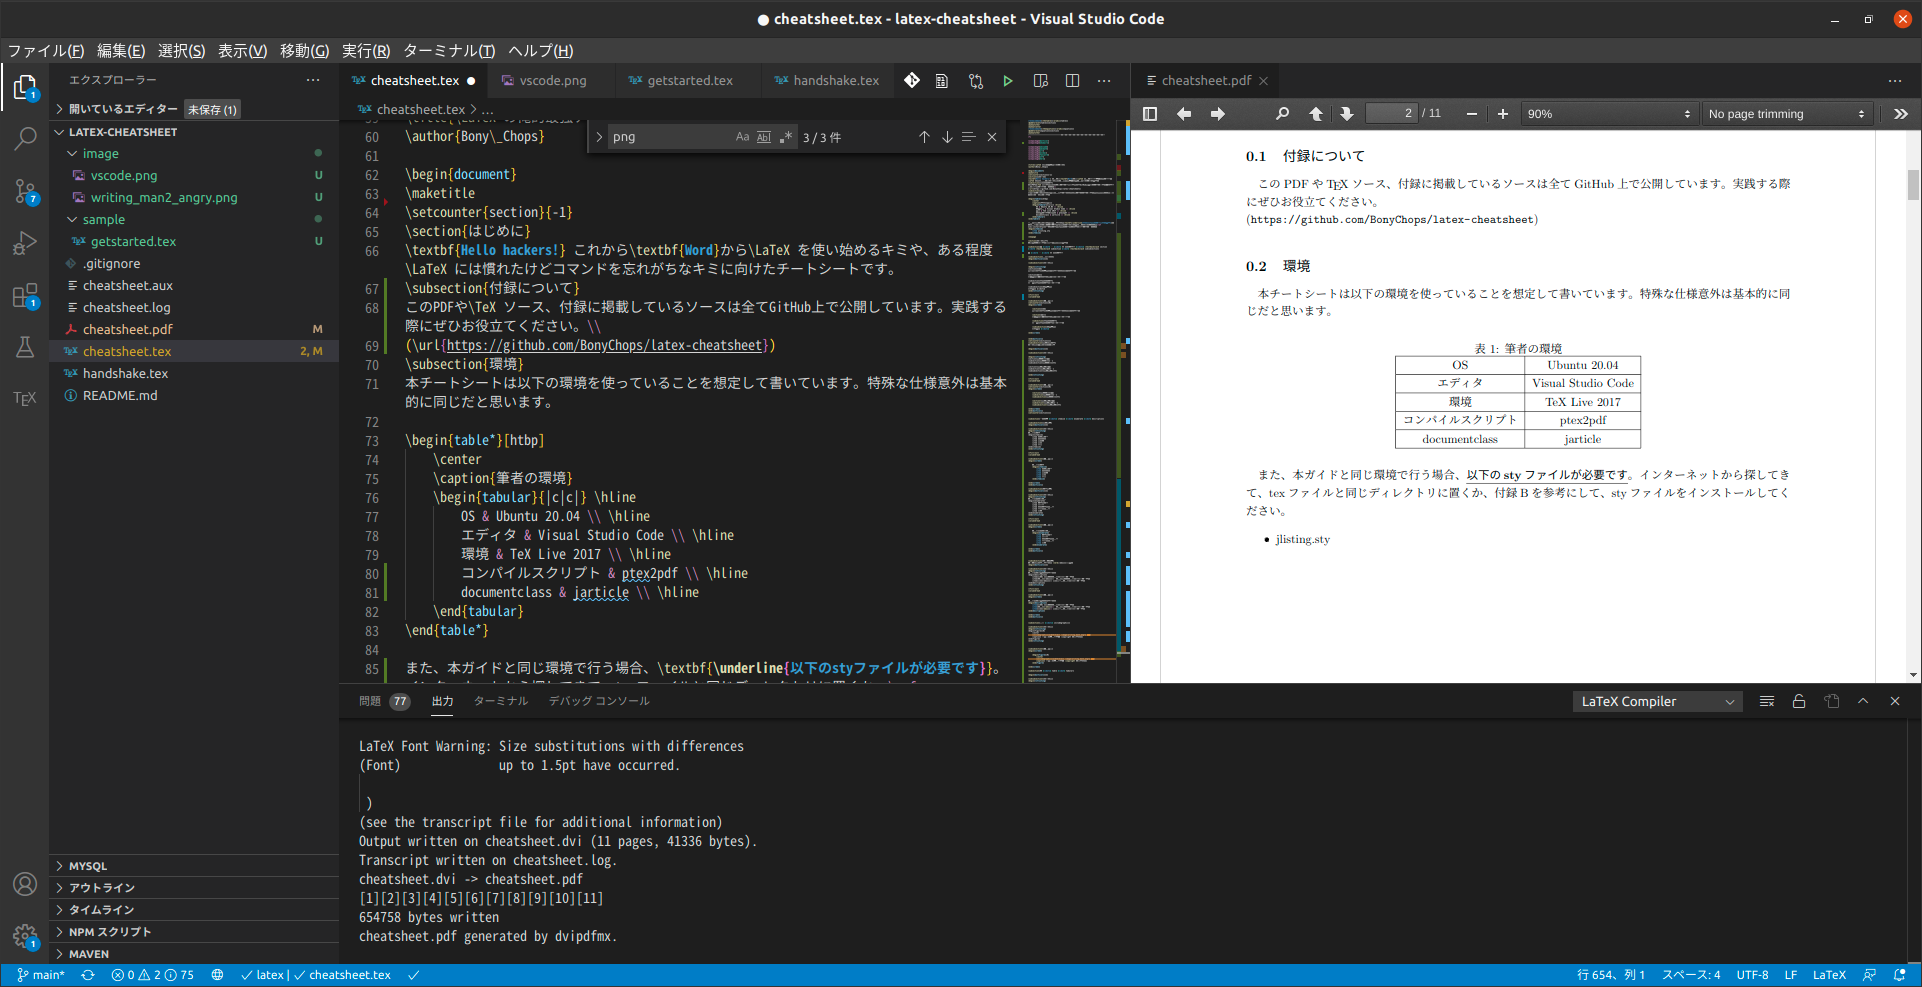
\includegraphics[width=16cm]{./image/vscode.png}
    \end{center}
\end{figure}
\TeX \ Worksと比較した時 $\cdots$
\begin{multicols*}{2}
    \subsection*{VSCodeで書くメリット}
    \begin{itemize}
        \item 複数のファイルを並べて置けるため、\textbf{PDFと\TeX ファイルを見比べながらできる!}
        \item コマンドを書く途中でサジェスト(候補)が出てくるため\textbf{すぐ書ける!間違えない!}
        \begin{figure}[H]
            \begin{center}
               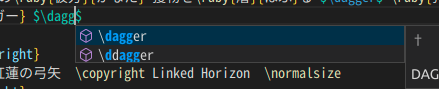
\includegraphics[width=8cm]{./image/vscode-dagger.png}
            \end{center}
        \end{figure}
        \item サイドバーにエクスプローラがあるため\textbf{複数ファイルがあっても把握しやすい!}
        \item エラーが(比較的)\textbf{わかりやすい!}
        \item コンパイルしなくても、カーソルをのせると\textbf{数式がプレビューされる!}
        \item コマンドが\textbf{色分けされて見やすい!}
        \item \textbf{Git}が使えるから、\textbf{レポートのバックアップも5秒以内!}(要ショートカット)
        \item \textbf{Discord}のRich Presenceで編集中のファイルを知ってもらえるから、\textbf{レポートやってますよ自慢ができる!}(需要は俺)



        \item VSCodeの\textbf{ショートカットが使える!}
        \begin{itemize}
            \item 文字を選択した後、\verb|(|, \verb|[|, \verb|{|, \verb|$|を入力すると、その記号(とその対になる記号)で囲ってくれる!
            \item マルチカーソルで\textbf{複数を一度に編集!}
            \item Git操作のショートカットを割り当てて、\textbf{音速Commit \& Push!}
            \item 自分でショートカットを\textbf{細かく決められる!}
        \end{itemize}
        \item ダークテーマだから\textbf{目に優しい!}(もちろんライトテーマもあるよ!好きなテーマを探そう)
        \item コンパイルが\textbf{早くなるらしい!}(諸説あり)
    \end{itemize}

\end{multicols*}

\subsection*{VSCodeで書くデメリット}
\begin{itemize}
    \item \TeX \ Worksにある、「PDFのここの部分と\TeX ソースのここが対応してる」を表示してくれる機能がない
    \item 最初のセットアップが少々面倒かもしれない
    \item VSCodeのPDFビューワに、クリックしたところだけをズームする機能がない(探せばあるかも?)
    \item なんだかんだもう\TeX \ Worksには戻れなくなるかもしれない
\end{itemize}

\subsection*{セットアップ}
\begin{enumerate}
    \item まずは\TeX \ Liveを通常通りインストールします(\TeX \ WorksはあってもなくてもOK)\\
    \quad すでにインストールしてある場合はここを飛ばしてください。バージョンはおそらくいくつでも大丈夫だと思います(2016-2019の動作確認済です)。インストール時にPATH(環境変数)を通すか聞かれた場合は、通すようにお願いしておきましょう。聞かれなかったり、お願いし忘れた場合は自分でパスを通します。詳しくは次。
    \item \TeX \ LiveのPATH(環境変数)が通っているか確認する\\
    \quad まず、コマンドプロンプト / ターミナルを開き\verb|ptex2pdf|と入力し\verb|Enter|。コマンドが見つからないと言われたら\ref{enu:path}を行う。
    \begin{enumerate}
        \item \label{enu:path}\TeX \ LiveのPATH(環境変数)を通す \\
        \quad 以下のPATHを通してください。通し方がわからない場合は、ここに書くと膨大になっちゃうので、こちらの記事をご覧ください。\\
        Windows 10でのパスの通し方 - Qiita\\
        (\url{https://qiita.com/BonyChops/items/a56ea9d0194a9992fd16})
        \begin{lstlisting}[caption=Windowsの場合のパス]
C:\texlive\{TeXの西暦}\bin\win32\
        \end{lstlisting}
    \end{enumerate}
    \item \textbf{VSCode}をインストールする \\
    \quad Windowsの場合、「VSCodeで開く」を追加する等のオプションはできるだけつけておいたほうが良いでしょう。
    \item \textbf{VSCode}に必要な拡張機能を入れておく\\
    \quad VSCodeを起動した後、左側のサイドバーにある拡張機能のアイコンをクリックすると、Marketplaceにアクセスすることができます。ここで、VSCodeスタータの皆様に、俺的イチオシ拡張機能を列挙しておきます。正直何もわからない場合は以下を全部入れてもいいと思います(☆は必須、それ以外は任意です)
    \begin{figure}[H]
        \begin{center}
           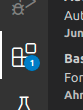
\includegraphics[width=2cm]{image/vscode-extension.png}
        \end{center}
    \end{figure}
    \begin{itemize}
        \item[☆] LaTeX Workshop - サジェストやコンパイル、色々やってくれる優れもの
        \item[☆] Snippet Generator - この後作るユーザースニペットがめちゃくちゃ簡単に作れるようになります
        \item Japanese Language Pack for Visual Studio Code - VSCodeが日本語になります
        \item Bracket Pair Colorizer 2 - 括弧の深度ごとに色分けされ、とにかくめちゃくちゃ見やすくなる
        \item Trailing Spaces - 行末に無駄なスペースが合った場合、そこが赤くなります
        \item zenkaku - 全角スペースを使っていた場合、そこが白くなります
        \item Discord Presence - Discordで自分の活動を自慢したい人向け
        \item Code Spell Checker - 英単語でスペルが間違っていた場合青色の波線で教えてくれる
        \item Settings Sync - Githubのアカウントをリンクして、インストールした拡張機能やその設定をバックアップ。これで別環境への移行も簡単にできます
        \begin{itemize}
            \item なんとそのうち\textbf{VSCode}が公式に設定のバックアップをできるようにするんだとか(しかも仕様はこの拡張機能とほとんど同じで,バックアップ先をMicrosoftアカウントや\GitHub Githubに指定可能)!興味がある人はこの拡張機能の代わりに公式のバックアップ機能を有効にしてもいいかもしれない(ただしまだプレビュー機能だそうです).
        \end{itemize}
        \item VS Code Counter - ワークスペース内のプロジェクトで、自分が何行書いたかを知れる
    \end{itemize}
    \item 設定を構成する\\
    \verb|Ctrl + Shift + P|もしくは\verb|F1|でコマンドを入力します。"\verb|settings json|"と入力し、 \text {\gt 基本設定: 設定(JSON)を開く}  を選択し,\GitHub \verb|bonychops/latex-cheetsheet|の\verb|settings/setting.json|の中身を貼り付けてください.
    \item ビルドしてみる\\
    とりあえずこれで最低限の設定は完了したので,試しにビルドしてみましょう.\verb|.tex|のファイルを作成してみて,いろいろ書いて,\verb|Ctrl + Alt + B|で正常にビルドできれば成功です.完成したPDFは\verb|Ctrl + Alt + V|で確認できます.
\end{enumerate}


\subsection*{ユーザースニペットを使いこなす}
早く書くために,スニペットを設定してみましょう.
\subsubsection*{(例)}
\verb|\screen| $\rightarrow$ \verb|Tab| $\downarrow$
\begin{lstlisting}
    \begin{screen}

    \end{screen}
\end{lstlisting}
\begin{enumerate}
    \item 画面左下歯車をクリック
    \item "\textbf{ユーザー スニペット}"
    \item "\textbf{新しい グローバル スニペット ファイル}"
    \item "\verb|latex|"
    \item \GitHub \verb|bonychops/latex-cheetsheet| の \verb|settings/snippet.json|を貼り付ける
\end{enumerate}

\subsection*{ユーザースニペットを自作する}
\TeX は便利だけど,毎回プリセット(\verb|\begin{document}より上の部分|)を書くのは大変 $\cdots$ と思っている人必見!さっきのスニペット機能を生かすと,毎回前回のレポートをコピーして $\cdots$ という無駄な時間をなくし,あなたの大切な時間を守れます!

\begin{enumerate}
    \item まず,設定したいプリセットを用意します.\ref{sec:env}から丸パクリでも良いです
    \item プリセットのソースファイルが選ばれている状態で\verb|Ctrl + Shift + P| $\rightarrow$ "\verb|Generate snippet|"
    \item "\verb|latex|"
    \item name: 適当な名前
    \item prefix: 呼び出す際のコマンドみたいなやつ
    \item description: 特にいらない
    \item 完成!
    \item テストしてみる: \\\verb|Ctrl + A| で選んだ後全部消してみて,何もない場所でprefixを打つと,登録したプリセットが現れます!
\end{enumerate}


\section{日本語 トラブルシューティングガイド}

\begin{thebibliography}{9}
    \bibitem{size} LaTeXコマンド集 - 文字サイズ \url{http://www.latex-cmd.com/style/size.html}
    \bibitem{style} LaTeXコマンド集 - 書体 \url{http://www.latex-cmd.com/style/style.html}
\end{thebibliography}


\end{document}